\chapter{Experimental}
\label{chap4}

This chapter first lists all tools used for testing. Then we describe how different types of glitch attacks will be simulated on the CV32E40S and CV32E40DC. The methodology behind the tests as well as a detailed description of how the tests are performed will be discussed. Lastly, this chapter introduces the general idea behind the architecture of the CV32E40DC. 

\section{Tools}
\label{sec:tools}

\begin{itemize}
    \item \textbf{Synthesis:} Cadence Genus 21\cite{cadence}
    \item \textbf{Simulation:} Cadence Xcelium 20.09.020\cite{xcelium}
    \item \textbf{Waveform analyzer:} SimVision (Part of Cadence Xcelium)\cite{simvision}
    \item \textbf{RISC-V Toolchain:} gcc-centos7-20230622\cite{toolchain}
\end{itemize}

\section{Methodology}
\label{sec:method}

The work in this project is based on the pre-existing code found in the CV32E40S repository \cite{cv32e40s_github}. Some design considerations had to be made when implementing CV32E40DC. As mentioned in \autoref{sec:xsecure} removing specific features of Xsecure is difficult due to them being heavily woven into many aspects of the core and the verification environment. Because of this, it was decided that only removing the PCH would be a good baseline for testing and comparison between the old and new architectures. This means that the CV32E40DC consists of two CV32E40S cores with PCH removed. To test that the architectures work they both run a "sanity" simulation of the code shown in \autoref{lst:sample_code} using \textit{Cadence Xcelium}.

Direct comparison between the cores is done by looking at the number of clock cycles needed to run the different test programs, as well as the area and power usage of the synthesized design. Synthesis is done using \textit{Cadence Genus} with a 45nm technology library. Reports of area and power usage are generated for comparison by the tool. The script used for synthesizing the designs and generating reports is shown in \autoref{lst:tcl}. Waveforms from the simulation of the cores are analyzed using \textit{SimVision}. The number of clock cycles needed to run the different test programs are counted using a built in feature of \textit{SimVision}. These comparisons are done mostly to give some understating of the resource usage, but for evaluating the effectiveness of the solution these metrics are not the most critical. As these cores are both meant to be used in applications where hardware security is of the utmost importance, they are often allowed to trade PPA for robustness. Both cores will therefore run two simple test programs shown in \autoref{lst:test_code} and \autoref{lst:coverage_test}. The former represents a secure boot protocol similar to the one shown in \autoref{fig:glitchable_code}. The latter represents an application with a lot of memory accesses. 

In the first test we will attempt to bypass a simulated secure boot protocol. As shown in \autoref{fig:glitchable_code} there are many ways that such a program can be exploited. However, because we only removed the PCH feature the glitching in this test will be restricted to the PC. This means we will only try to do instruction skipping, and no resetting of register values or status registers for conditional branches. In the second test we wish to investigate the fault detection coverage of both cores by glitching the values on the OBI data-bus. This test purposefully attacks parts of the core that are not explicitly covered by features from \textit{Xsecure}. This way it will be possible to see whether the CV32E40DC indeed offers extra fault coverage as a trade off to the increased area and power usage. 


Both cores execute the same instructions at different times due to the absence of the PCH feature in CV32E40DC. Consequently, fault injection must therefore also occur at distinct times for each core. However, within each core, faults are injected at a fixed time stamp for each respective test. The behaviour of the simulator and cores are deterministic. This means that each test will theoretically only need to run once as the result will always be the same. Despite this, every test is run at least twice to make sure of this.

We assume some external logic will handle whenever a glitch is detected. This means that the quality of a core is not determined by whether a glitch attack is successful\footnote{Meaning for example that a restricted part of the code is accessed or a wrong value is calculated.}. Instead it is solely determined by whether or not the core is able to detect an error. 

\subsection{Simulating glitch attacks}
\label{subsec:sim_glitch}

Real glitch attacks as described in \autoref{sec:glitch_attacks} are done by tampering with some external stimuli to a device, like the clock, voltage or temperature. Using the same attacks in simulation is both complicated and often not possible. However, to simulate an attack, a \textit{glitch injector} module was implemented. The code for this module is shown in \autoref{lst:glitch_injector}. During simulation the module is always running and the output is controlled by the \textit{enable, enable\_specific} and \textit{rst\_n} signals as shown in \autoref{tab:module_output}. Any signal that we wish to glitch can then be forced at a specific time to hold the output value of the \textit{glitch\_injector}.

\begin{table}[h]
\centering
\caption{Glitch Injector output based on control signals.}
\label{tab:module_output}
\begin{tabular}{ccccc}
\toprule 
\rowcolor{black!20} \textbf{enable} & \textbf{enable\_specific} & \textbf{rst\_n} & \textbf{in} & \textbf{out} \\
\midrule
0 & 0 & x & x & x \\
\rowcolor{black!20} 1 & 0 & 1 & 0 & Random \\
1 & 0 & 1 & 1 & Random \\
\rowcolor{black!20} 1 & 1 & 1 & x & Specific \\
\bottomrule
\end{tabular}
\end{table}

\begin{lstlisting}[caption={SystemVerilog code for the glitch\_injector module}, label=lst:glitch_injector, language=verilog]
module cv32e40s_glitch_injector 
#(
parameter BIT_LENGTH = 1, 
parameter SPECIFIC = {BIT_LENGTH{1'b0}}
)
(
    output  logic [0:BIT_LENGTH-1]      out,
    input   logic [0:BIT_LENGTH-1]      in,
    input   wire                        clk,
    input   wire                        rst_n,
    input   wire                        enable,
    input   wire                        enable_specific    
);

always_ff @ (posedge clk, negedge rst_n) begin 
    if (rst_n == 1'b0) begin 
        out $<=$ 0;
    end else begin
        reg [BIT_LENGTH-1:0] random_out; 

        if (enable_specific) begin
            out $<=$ SPECIFIC;
        end else if (enable && !enable_specific) begin
            random_out = $\$$urandom;
            out $<=$ random_out; 
        end else
            out $<=$ in;  
    end
end
endmodule
\end{lstlisting}

While this module allows for fault injection, there are still some complications related to performing a successful attack that must be addressed. As mentioned in \autoref{sec:non_invasive}, effective glitch attacks require very precise timing. While doing this in simulation is a lot simpler than doing it on a physical device, we still need to "reverse engineer" our program to figure out where to do fault injection. The steps for performing an attack are described below:

\begin{enumerate}
    \item Write high level C code containing some vulnerability that can be exploited. 
    \item Compile the code with no optimization to make relationship between C and Assembly as close as possible.
    \item Analyse the Assembly and identify the instruction(s) that can be glitched.
    \item Simulate the core running the code without any fault injection to log all executed instructions. 
    \item Analyze the log file to figure out at what time the glitchable instruction was executed. The log file only logs at what time the instruction reached the WB stage, meaning we must subtract 1-3 clock periods depending on which part of the pipeline we wish to introduce the glitch. 
    \item Rerun simulation with fault injection and verify that the expected glitch occurs at the right time. If not, redo step 5 with different timing. 
\end{enumerate}

\subsection{Skipping instructions}
\label{subsec:skip_instr}

In a real system, manipulating the program counter to specific values can be challenging. However, utilizing voltage- or clock-glitching techniques allows for the disruption of the normal logic behavior responsible for incrementing the program counter. This interference enables the incrementation of the pointer multiple times, effectively skipping one or more instructions. Consequently, if an attacker possesses knowledge of the execution sequence, they can strategically skip branches or jumps, gaining unauthorized access to restricted sections of the code. This type of attack can be simulated with the \textit{glitch\_injector} by setting the output of the module equal to a specific value. 

In cases where the attacker has limited insight into the instruction sequence but has access to the system's boot-loader, an alternative method for instruction skipping exists. By inserting numerous 'NOP' instructions before the targeted restricted code area, the attacker can 'scramble' the program counter, and have an increased probability of landing on a 'NOP'. From this instruction the system continues sequential execution, eventually reaching the desired restricted code. This type of attack can be simulated with the \textit{glitch\_injector} by setting the output of the module equal to a random value. However, this is very time consuming and is therefore not within the scope of this project. These types of attacks are instead simulated by attempting to jump from the beginning of the 'main' function directly to the restricted code. 

\section{Simulating instruction skipping}
\label{sec:sim_instr_skip}

Because the tests are restricted to instruction skipping, it limits the potential ways such a small program can be exploited. However, the tests shown in \autoref{tab:instr_skip_test} will be run on the code shown in \autoref{lst:test_code}. Most, if not all, of the code in the test is somewhat redundant. Because of this, the code is compiled with the '-O0' flag. This way no optimizations are applied and the C-code and RISC-V assembly are as closely related as possible. The assembly for the test program is shown in \autoref{lst:asm_instr_skip}. 

\begin{lstlisting}[caption={Test code for simulating instruction skip.}, label=lst:test_code, language=C++]
int main(int argc, char *argv[])
{
    int result_code = 0;

    /* Count to avoid actual infite loop */
    unsigned int count = 0;

    /* Get error result code */
    result_code = boot_go();

    if (result_code != 0) {
      while(1) {
       	if (count > 10)	{
          printf("Exiting...\n");
       	  return EXIT_SUCCESS;
        }
        count++;
      }
    }

    printf("Glitched out of loop\n");
    do_boot();
    return EXIT_FAILURE;
}
\end{lstlisting}

\begin{table}[h]
\centering
\caption{Instruction skipping tests.}
\label{tab:instr_skip_test}
\begin{tabular}{m{2.5cm}m{3.5cm}m{7.5cm}}
\toprule 
Line in C code & ASM instruction & Expected outcome \\
\midrule
\rowcolor{black!20} \textbf{9} & c.jal 418 $\langle$boot\_go$\rangle$ & Skipping this instruction means that the value of '-1' from the 'boot\_go()' function is never stored in the 'result\_code' register. The program then never enters the scope of the conditional statement. \\
\textbf{12} & c.j 458 $\langle$main+0x20$\rangle$ & Skipping the jump instruction that keeps the 'while(1)' loop repeating will glitch out of the scope of the loop and execute the 'do\_boot()' function.  \\
\rowcolor{black!20} \textbf{Any line} & Any instruction & From any point in the code it is potentially possible to glitch directly to the address of the 'do\_boot()' function. The real danger of this happening is discussed in \autoref{subsec:skip_instr}. \\
\bottomrule
\end{tabular}
\end{table}

\section{Coverage tests}
\label{sec:coverage_test}

While it is important to verify whether the CV32E40DC can replace the existing security features of \textit{Xsecure}, it does not explore one of the main advantages which is fault coverage. In order to test this, we will introduce glitches in areas that are not specifically covered by \textit{Xsecure}. One such area is the data-bus going to the data-memory during a load or store instruction. If this is attacked with only one core, the wrong data might stay in the memory undetected and faults can propagate to other parts of the execution sequence. With two cores any discrepancy between the loaded or stored data can be detected before faults disrupt the system. 

These types of attacks pose a real threat as data-buses are often long because they have to go between different modules, and require a large area if the bus is wide. This large area makes it easy for an attacker to target the bus with something like EMFI if they have some knowledge of the chip layout. Voltage and clock glitches can also potentially disrupt the data on a bus. 

In order to test the fault coverage of both cores, the test program shown in \autoref{lst:coverage_test} is used. This code runs a simple function that calculates the 20th Fibonacci number. The function uses no recursion and the code is compiled without optimization. This is to make the C-code and Assembly as closely related as possible. Each line in the loop body between line 6 and 10 translates to at least one load and store instruction. Glitching any of these instructions will lead to a similar result. Because of this we only glitch the instructions corresponding to line 7 in the code. \autoref{tab:coverage_test} shows the tests that will be run. 

%Because disrupting the \textit{load} or \textit{store} instructions in either one of the lines in the code leads to a similar outcome, the glitches will only be applied to the instructions corresponding to ine \textbf{7}.

\begin{lstlisting}[caption={Test code for simulating glitch in address-bus.}, label=lst:coverage_test, language=C++]
int main(int argc, char *argv[])
{
    int prev = 0;
    int current = 1;

    for (int i = 1; i < 20; i++) {
        int next = prev + current;
        prev = current;
        current = next;
    }

    if (current == 6765) {
        printf("No glitch detected\n");
        return EXIT_SUCCESS;
    }
    printf("Glitch detected\n");
    return EXIT_FAILURE;
}
\end{lstlisting}

\begin{table}[h]
\centering
\caption{Fault coverage tests.}
\label{tab:coverage_test}
\begin{tabular}{m{2.5cm}m{3.5cm}m{7.5cm}}
\toprule 
Line in C code & ASM instructions & Expected outcome \\
\midrule
\rowcolor{black!20} \textbf{7} & \makecell{lw	x14,-20(x8) \\ lw x15,-24(x8) \\ c.add x15,x14 \\ sw x15,-32(x8)} & Disrupting either the \textit{lw} or \textit{sw} instructions should lead to the wrong result at the end of the loop.\\
% \textbf{8} & \makecell{lw x15,-24(x8) \\ sw x15,-20(x8)} & Disrupting either the \textit{lw} or \textit{sw} instruction should lead to the wrong result at the end of the loop. \\
% \rowcolor{black!20} \textbf{9} & \makecell{lw x15,-32(x8) \\ sw x15,-24(x8)} & Disrupting either the \textit{lw} or \textit{sw} instruction should lead to the wrong result at the end of the loop.\\
\bottomrule
\end{tabular}
\end{table}

\section{Implementing the CV32E40DC}
\label{sec:dualcore}

The proposed dual-core architecture is straight forward to implement. All that is needed is to connect two cores with synchronization registers at appropriate places. Choosing the correct granularity for comparisons is however important. At the highest level, comparing only the output of both cores is an option. Comparison would then have to be done on the OBI data bus. For the end-user application, this would be the most natural way to do it as the details of what has glitched is far less important than simply detecting that an error has occurred. However, for analyzing the effects of glitch attacks on a system in more detail, a more fine grained approach is needed. The extreme counterpart to only comparing the output would be to compare all wires and registers. This would allow the user to determine the exact location of an error, but at the cost of adding a lot of extra hardware. 

%This way of implementing the comparisons can also be argued against as it goes against one of the principal ideas of using a dual-core lockstep mechanism: simplicity of implementation. 

As the purpose of this project is to analyze the effectiveness of the dual-core lockstep mechanism, some granularity is needed. However, knowing exactly which wire or register bit has glitched will not be necessary. This would also add a lot of extra work for simply connecting everything. Therefore, synchronization registers where comparison happens will be connected to the input signals going to different stages of the pipeline as well as to every input and output signal of the core going to the OBI interfaces. From this data it is then possible to detect a glitch and give the user some information about exactly where in the pipeline the fault occurred.

As an added bonus from using synchronization registers is that the two cores are offset from each other by a clock cycle. This way, in the unlikely event that an attacker manages to glitch the two cores in precisely the same way at the same time, they now need to do it in a highly synchronized manner. This significantly increases the complexity of the attack. The deliberate offset between the cores introduces a form of time diversity, making it more challenging for an attacker to exploit vulnerabilities using clock glitches or other timing-based attacks. These additional security measures enhance the system's resistance to fault injection attacks and improve its overall robustness.

The top level block diagram for the dual-core lockstep setup is shown in \autoref{fig:dual_block}. The red blocks represent a stage in the pipeline. The yellow rectangles are the registers between the different pipeline stages. The dark blue blocks are the data- and instruction-memory interfaces. The light blue blocks are the LSU modules responsible for communicating with the data interface. Each purple block represents a synchronization register that delays a signal one clock cycle. The green blocks represent logic dedicated to comparing the signals from both cores. If any of the comparisons fail, one of four bits on the \textit{alert\_compare\_o} wire will be set to '1'. Which bit is set tells the user which one of the comparisons that failed.  

\begin{figure}[ht!]
    \centering
    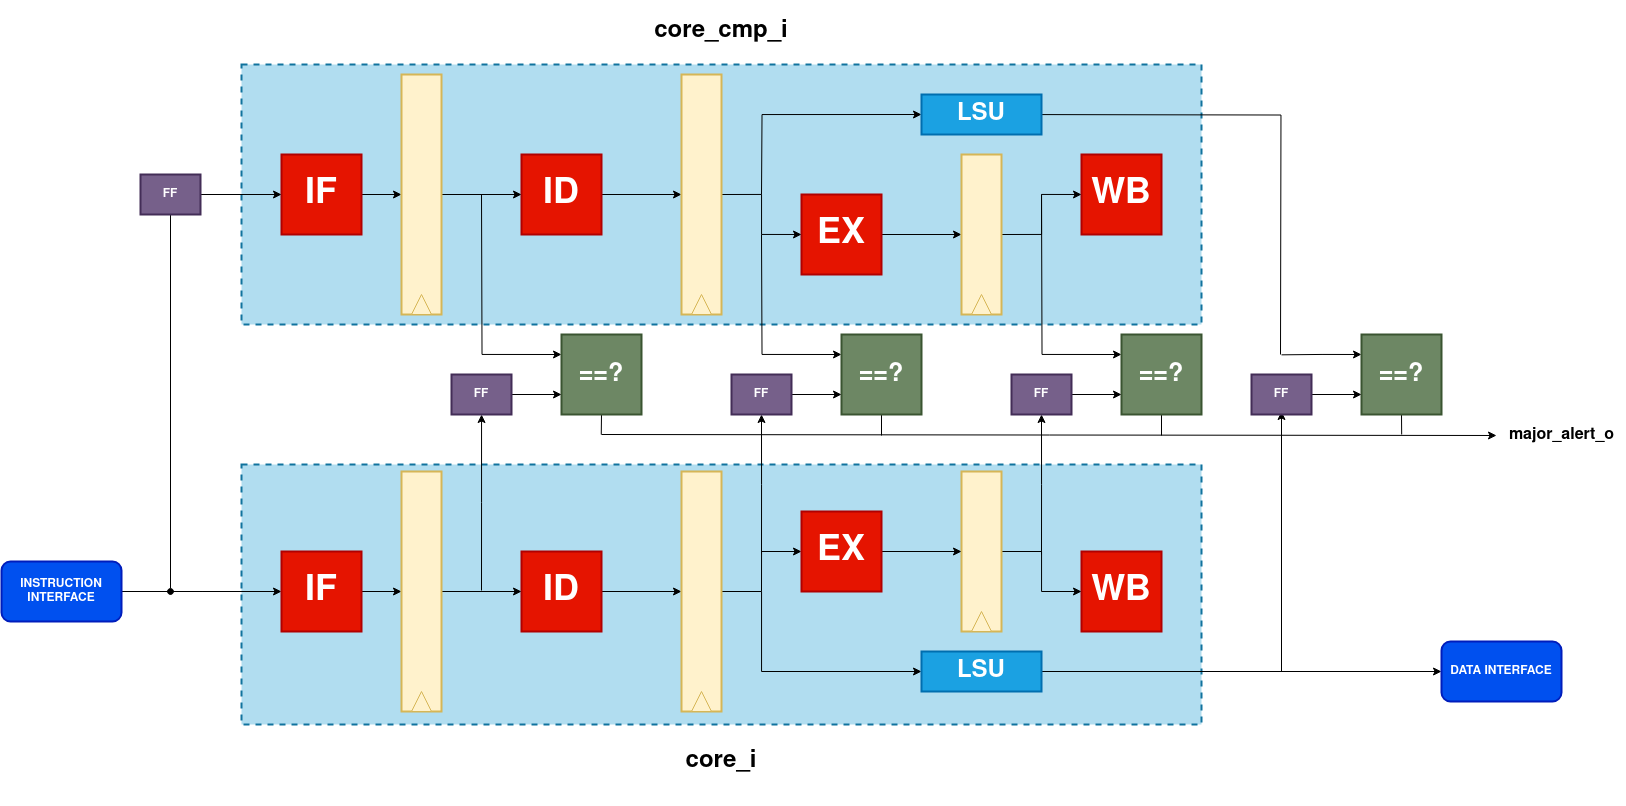
\includegraphics[width=\textwidth]{docs/images/dual_cores-block.png}
    \caption{Block diagram cv32e40s dual-core lockstep mechanism.}
    \label{fig:dual_block}
\end{figure}

Parts of the implementation of CV32E40DC are shown in \autoref{lst:dc_code}. This is a slightly modified and extended version of the \textit{cv32e40s\_core.sv} code found in \cite{cv32e40s_github}. The major changes are the removal of the PCH feature, adding the pipeline stages as outputs and the instantiation of a second core. All the same inputs and outputs are declared for both cores. A synchronization register is made for each of these signals. The signals from both cores are compared in four separate statements. The first comparison is between all the output signals that exist in the unmodified CV32E40S. The next three comparisons are of the different pipeline stages. This way we can differentiate between an error in the pipeline or one occurring somewhere in the normal outputs. 

Because all inputs and outputs of the core remain the same (with the exception of the output pipeline signals) we can easily connect it to the pre-existing verification framework. \autoref{lst:dc_wrapper} shows the instantiation of the CV32E40DC and a glitch injector module in the test bench.
